\thispagestyle{hoccungpinone}
\pagestyle{hoccungpi}
\everymath{\color{hoccungpi}}
\graphicspath{{../hoccungpi/pic/}}
\blfootnote{\color{hoccungpi}\color{hoccungpi}$^1$Sinh viên Trường ĐH Sư phạm TP.HCM.}
\begingroup
\AddToShipoutPicture*{\put(0,616){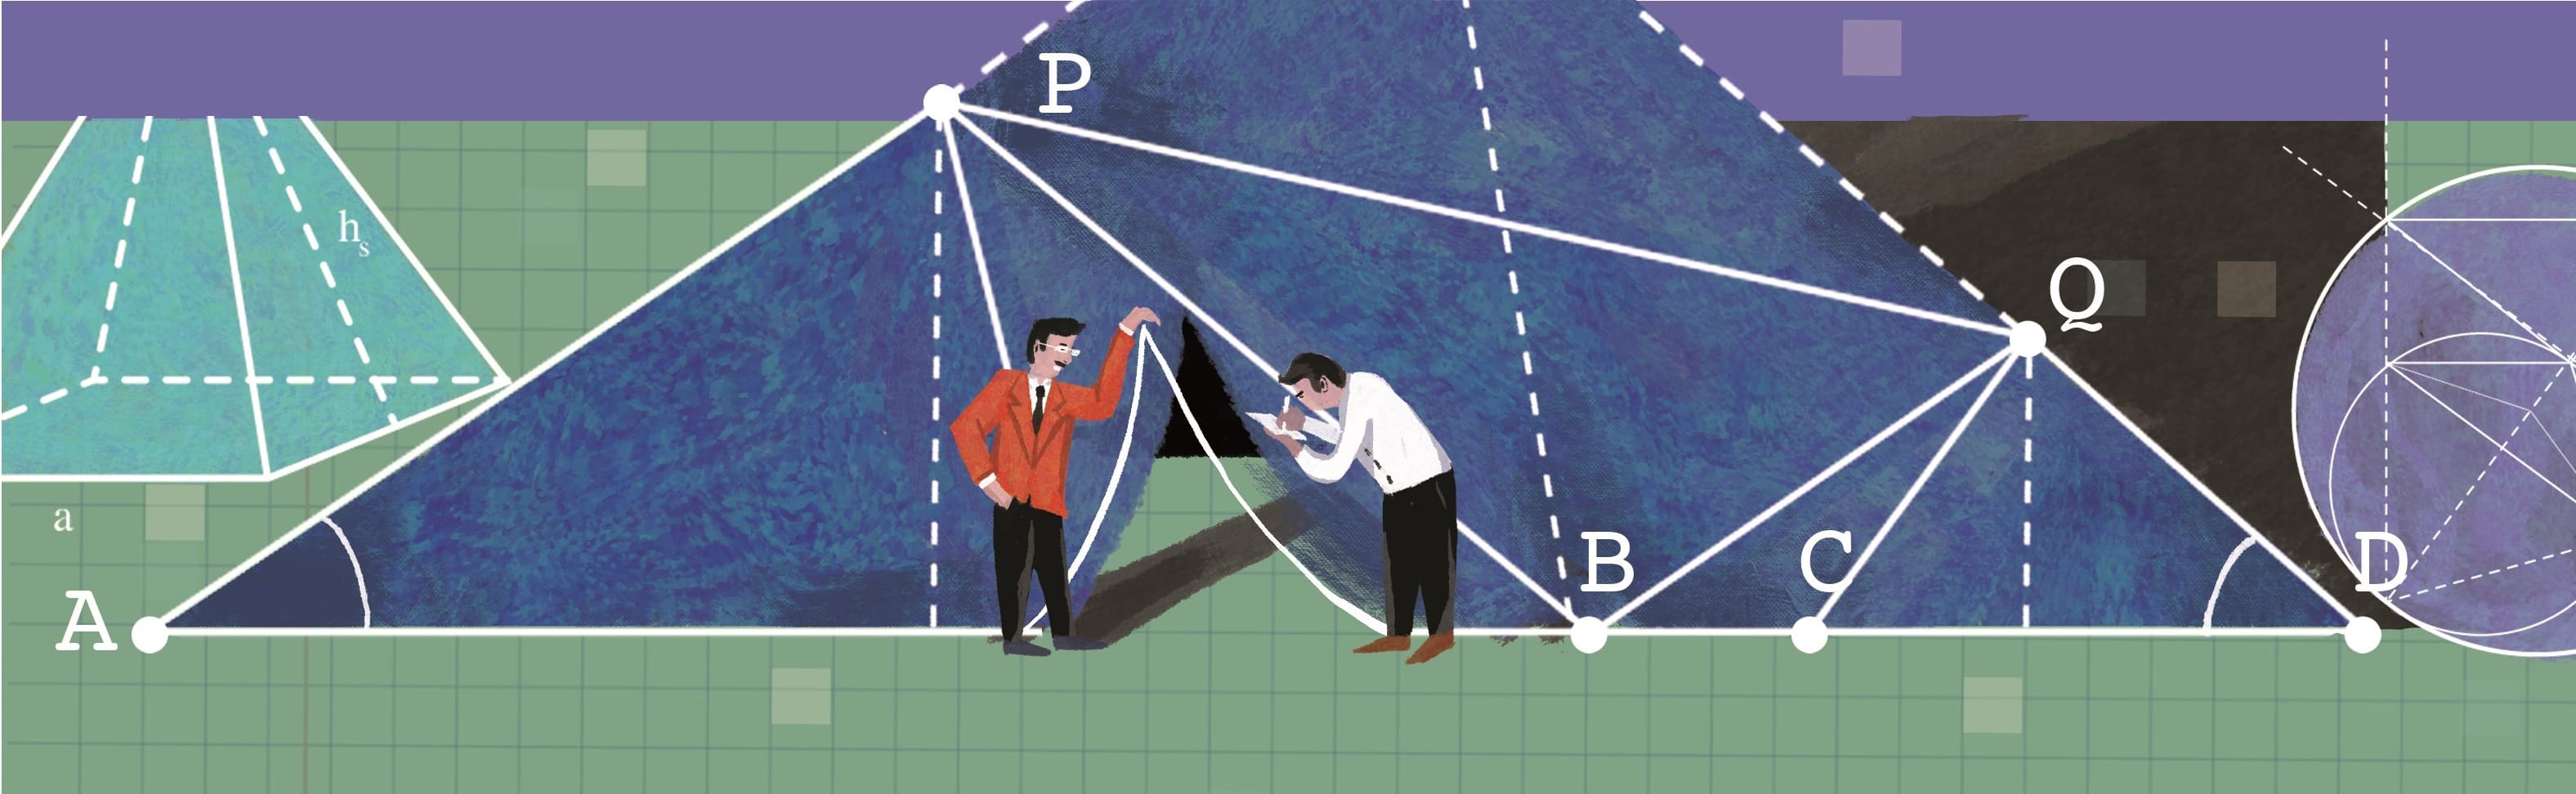
\includegraphics[width=19.3cm]{../bannerhoccungpi}}}
\AddToShipoutPicture*{\put(56,522){
\includegraphics[scale=1]{../tieude.pdf}}}
\centering
\endgroup
\vspace*{190pt}

\begin{multicols}{2}
	$\pmb{1.}$	\textbf{\color{hoccungpi}Giới thiệu}
	\vskip 0.1cm
	Những bài toán phương trình hàm trên tập hợp số thực dương đã không còn quá xa lạ đối với các bạn học sinh chuyên Toán và ngày càng xuất hiện nhiều hơn trong các đề thi Olympic dạo gần đây. Trong số đó, có thể kể đến bài toán nằm trong đề thi chọn đội tuyển Quảng Ninh tham dự kỳ thi học sinh giỏi cấp quốc gia môn Toán (VMO) năm học $2022-2023$ dưới đây: 
	\vskip 0.1cm
	\textbf{\color{hoccungpi}Bài toán:} [Quảng Ninh $2022 - 2023$]
	\vskip 0.1cm
	Tìm tất cả hàm số $f: \mathbb{R^+} \to \mathbb{R^+}$ thỏa mãn: 
	\begin{align*}
		f(3f(x) + 3y) = f(3x + y) + 2y,\tag{$1$}
	\end{align*}
	với mọi $x,y$ thuộc $\mathbb{R^+}$.
	\vskip 0.1cm
	Bài viết này bàn về bảy lời giải cho bài toán trên qua đó giới thiệu cho bạn đọc những kỹ năng, kỹ thuật cơ bản để giải quyết những bài toán phương trình hàm trên tập hợp số thực dương nói riêng và những bài toán phương trình hàm nói chung.
	\vskip 0.1cm
	$\pmb{2.}$	\textbf{\color{hoccungpi}Lời giải bài toán}
	\vskip 0.1cm
	Giả sử rằng tồn tại hàm $f$ thỏa mãn các yêu cầu bài toán. Trước hết ta có các nhận xét sau:
	\vskip 0.1cm
	\textbf{\color{hoccungpi}Nhận xét $\pmb1$.} $f(x) \ge x, \forall x > 0$.
	\vskip 0.1cm   
	\textit{Chứng minh.}  Giả sử tồn tại $x_0 > 0$  sao cho $f(x_0) < x_0$. Trong ($1$) cho $x = x_0$  và  $y = \dfrac{3\left(x_0 -f(x_0)\right)}{2}$ ta được: 
	\begin{align*}
		3({x_0} - f({x_0})) = 0 \Rightarrow f({x_0}) = {x_0}, \text{ vô lý!}
	\end{align*}
	Do đó $f(x) \ge x, \forall x > 0$.
	\vskip 0.1cm  
	\textbf{\color{hoccungpi}Bình luận.}  Lý do nào khiến ta nghĩ ra được đánh giá trên? Quan sát phương trình ($1$), ta mong muốn triệt tiêu $f$  ở cả hai vế bằng cách lựa chọn $x, y > 0$  sao cho: 
	\begin{align*}
		3f(x) + 3y = 3x + y.
	\end{align*}
	Chuyển vế, thu được $y = \dfrac{3\left(x - f(x)\right)}{2}$.  Ý đồ của ta sẽ thành công nếu ta tìm được $x > 0$  sao cho  $f(x) < x$. Tuy nhiên với $x,y$  như vậy thì ($1$) trở thành: $2y = 0$, vô lý! Do đó phép chọn này không thể thực hiện được, và vì thế điều ngược lại là $f(x) \ge x , \forall x > 0$  ắt phải đúng!
	\vskip 0.1cm
	\textbf{\color{hoccungpi}Nhận xét $\pmb2$.} $f$ là đơn ánh.
	\vskip 0.1cm
	\textit{Chứng minh.}  Giả sử tồn tại $a > b > 0$  sao cho $f(a) = f(b) = c$.  Trong ($1$) lần lượt cho $x = a $ và $x = b$  thì được: 
	\begin{align*}
		f(y + 3a) + 2y &= f(3y + 3c) \\
		&= f(y + 3b) + 2y,\forall y > 0.
	\end{align*}
	Suy ra: 
	\begin{align*}
		f(y + 3a) = f(y + 3b),\forall y > 0.
	\end{align*}
	Từ đây thay $y$  bởi $y - 3b$  và đặt $T = 3a - 3b > 0$  thì được:
	\begin{align*}
		f(y) = f(y + T),\forall y > 3b.
	\end{align*}
	Bằng quy nạp ta chứng minh được: 
	\begin{align*}
		f(y) = f(y + nT),\forall y > 3b,n \in \mathbb{N^*}.
	\end{align*}
	Trong đẳng thức trên chọn $y = 3b + 1$  và sử dụng \textbf{\color{hoccungpi}Nhận xét $\pmb1$} ta được: 
	\begin{align*}
		f(3b + 1) &= f(3b + 1 + nT) \\
		&\ge 3b + 1 + nT,\forall n \in \mathbb{N^*}
	\end{align*}
	Đến đây cho  $n \to +\infty$ ta thu được điều vô lý. Do vậy $f$  là đơn ánh.
	\vskip 0.1cm
	\textbf{\color{hoccungpi}Bình luận.} Đối với những bài toán tìm hàm  $f: \mathbb{R^+} \to \mathbb{R^+}$, ta thường chú ý đến tính đơn điệu, đơn ánh, tuần hoàn, bị chặn, cộng tính, \ldots\, của hàm  $f$. Đặc biệt, kỹ thuật phản chứng, xây dựng hàm tuần hoàn nhằm chứng minh $f$  đơn ánh đã trở thành ý tưởng quen thuộc khi giải quyết những bài toán dạng này.
	\vskip 0.1cm 
	Sau khi thu được hai nhận xét trên, tôi xin trình bày bảy lời giải cho bài toán gốc như sau:
	\vskip 0.1cm
	\textbf{\color{hoccungpi}Cách $\pmb{1}$:}
	\vskip 0.1cm
	Trong ($1$) thay $x$  bởi $3f(x) + 3z$ thì được: 
	\begin{align*}
		&f(3f(3f(x) + 3z) + 3y) \\
		&=f(9f(x) + 9z + y) + 2y,\forall x,y,z > 0
	\end{align*}
	suy ra, theo ($1$)
	\begin{align*}
		&f(3f(3x + z) + 6z + 3y) \\
		=&f(9f(x) + 9z + y) + 2y,\forall x,y,z > 0
	\end{align*}
	suy ra, theo ($1$)
	\begin{align*}
	&f(3(3x + z) + 2z + y) + 4z + 2y \\
	= &f(9f(x) + 9z + y) + 2y,\forall x,y,z > 0
	\end{align*}
	suy ra
	\begin{align*}
		&f(9x + 5z + y) + 4z \\
		&= f(9f(x) + 9z + y),\forall x,y,z > 0. \tag{$2$}
	\end{align*}
	Đến đây thay $y$  và $z$  bởi $\dfrac{z}{2}$  ta được: 
	\begin{align*}
		f(9x + 3z) + 2z 
		= f(9f(x) + 5z),\forall x,z > 0
	\end{align*}
	suy ra
	\begin{align*}
		f(3(3x + \frac{{2z}}{3}) + z) + 2z =f(9f(x) + 5z),
	\end{align*}
	với mọi $x,z > 0$.
	Suy ra, theo ($1$)
	\begin{align*}
		f(3f(3x + \frac{{2z}}{3}) + 3z) = f(9f(x) + 5z),
	\end{align*}	
	với mọi $x,z > 0$. Mặt khác $f$  là đơn ánh nên: 
	\begin{align*}
		3f(3x + \frac{{2z}}{3}) + 3z = 9f(x) + 5z,\forall x,z > 0.
	\end{align*}
	Dẫn đến:
	\begin{align*}
		f(3x + \frac{{2z}}{3}) = 3f(x) + \frac{{2z}}{3},\forall x,z > 0.
	\end{align*}
	Đến đây thay $z$  bởi $\dfrac{9z}{2}$  thì được:
	\begin{align*}
		f(3x + 3z) = 3f(x) + 3z,\forall x,z > 0.
	\end{align*}
	Trong đẳng thức trên hoán đổi vị trí của $x$  và $z$ cho nhau ta được: 
	\begin{align*}
		&3f(z) + 3x = 3f(x) + 3z,\forall x,z > 0\\
		\Rightarrow &f(x) - x = f(z) - z,\forall x,z > 0.
	\end{align*}
	Suy ra: 
	\begin{align*}
		f(x) = x + C,\forall x > 0 \text{ ($C$ là hằng số).}
	\end{align*}
	Thay công thức trên vào ($1$) ta được: 
	\begin{align*}
		&3x + 3y + 4C = 3x + 3y + C,\forall x,y > 0.
	\end{align*}
	Vậy $C = 0$. Vậy bài toán đã cho có duy nhất một nghiệm hàm là $f(x) = x, \forall x >0$.
	\vskip 0.1cm
	\textbf{\color{hoccungpi}Cách $\pmb2$:} (tiếp nối từ ($2$))
	\vskip 0.1cm 
	Trong ($2$) cho $z = x$ thì được: 
	\begin{align*}
	f(14x + y) + 4x = f(9f(x) + 9x + y),
	\end{align*}
	với mọi $x,y > 0$. Đến đây thay $y$  bởi $y - 14x$  thì được: 
	\begin{align*}
		f(y) + 4x = f(y + 9f(x) - 5x), 
	\end{align*}
	với mọi $x > 0,y > 14x$.
	\vskip 0.1cm
	Với mọi  $x > 0$, đặt  $g(x) = 9f(x) - 5x \ge 4x > 0.$ Lúc này đẳng thức trên trở thành: 
	\begin{align*}
		&f(y) + 4x \\
		= &f(y + g(x)),\forall x > 0,y > 14x. \tag{$3$}
	\end{align*}
	Đến đây thay $x$  bởi $x + z$  thì được: 
	\begin{align*}
		f(y + g(x + z))
		= &f(y) + 4x + 4z\\
		\mathop  = \limits^{(3)} &f(y + g(x)) + 4z\\
		\mathop  = \limits^{(3)} &f(y \!+\! g(x) \!+\! g(z)),
	\end{align*}
	với mọi $ x,z > 0,y > 14(x + z)$.
	Lại có $f$ là đơn ánh nên: 
	\begin{align*}
		y + g(x + z) = y + g(x) + g(z),
	\end{align*}
	với mọi $x,z > 0,y > 14(x + z).$ Dẫn đến: 
	\begin{align*}
		g(x) + g(z) = g(x + z),\forall x,z > 0.
	\end{align*}
	Như vậy $g: \mathbb{R^+} \to \mathbb{R^+}$  và $g$ cộng tính trên $\mathbb{R^+}$  nên $g(x) = xg(1),\forall x > 0.$  Nói cách khác, 
	\begin{align*}
		9f(x) - 5x = xg(1),\forall x > 0,
	\end{align*}
	suy ra
	\begin{align*}
		f(x) = \alpha x,\forall x > 0. \text{ ($\alpha$ là hằng số)}
	\end{align*}
	Thay công thức trên vào ($1$) ta được: 
	\begin{align*}
		\alpha (3\alpha x + 3y) = \alpha (3x + y) + 2y,\forall x,y > 0,
	\end{align*}
	suy ra $\alpha = 1.$
	Vậy bài toán đã cho có duy nhất nghiệm hàm  $f(x)= x, \forall x > 0$.
	\vskip 0.1cm
	\textbf{\color{hoccungpi}Cách $\pmb3$:} (tiếp nối từ ($3$))
	\vskip 0.1cm 
	Trong ($1$) thay $y$ bởi $2y$ thì được: 
	\begin{align*}
		f(3f(x) \!+\! 6y) \!=\! f(3x \!+\! 2y) \!+\! 4y,\forall x,y > 0
	\end{align*}
	suy ra, theo ($3$)
	\begin{align*}
		f(3f(x) + 6y) = f(3x + 2y + g(y)),
	\end{align*}
	với mọi $y > 0,3x + 2y > 14y.$ 
	\vskip 0.1cm
	Lại có  $f$ là đơn ánh nên: 
	\begin{align*}
		3f(x) + 6y = 3x + 2y + g(y),
	\end{align*}
	với mọi $y > 0,x > 4y.$
	Nói cách khác, 
	\begin{align*}
		f(x) - x = 3(f(y) - y),
	\end{align*}
	với mọi $y > 0,x > 4y.$
	\vskip 0.1cm
	Với mọi $x > 0$, đặt $h(x) = f(x) - x$. Từ đẳng thức trên ta có ngay: 
	\begin{align*}
		h(x) = 3h(y),
	\end{align*}
	với mọi $y > 0,x > 4y.$
	\vskip 0.1cm
	Giả sử ta cố định $y > 0$  thì lập tức $h$ là hàm hằng trên khoảng $(4y, + \infty)$. Bằng cách cho $y \to 0^+$  ta sẽ thu được $h$ là hàm hằng trên toàn bộ khoảng $(0 , + \infty)$. Dựa trên phân tích này, ta có thể giải tiếp bài toán như sau:
	\vskip 0.1cm
	Lấy $x > z > 0$  tùy ý. Ta sẽ chứng minh $h(x) = h(z)$.
	\vskip 0.1cm 
	Thật vậy, chọn $y = \dfrac{z}{5}$  thì $x > 4y$  và  $z > 4y$. Khi đó $h(x) = 3h(y) = h(z)$.  Do đó  $h$ là hàm hằng trên $\mathbb{R^+}$. Nói cách khác, 
	\begin{align*}
		f(x) - x = C,
	\end{align*}
	với mọi $x > 0$. $C$ là hằng số.
	\vskip 0.1cm
	Thay công thức trên vào ($1$) ta tìm được: $C = 0.$
	\vskip 0.1cm
	\textbf{\color{hoccungpi}Cách $\pmb4$:} (tiếp nối từ ($3$))
	\vskip 0.1cm     
	Điểm mấu chốt của \textbf{\color{hoccungpi}Cách $\pmb2$} và \textbf{\color{hoccungpi}Cách $\pmb3$} là dựa vào phương trình ($3$) và tìm cách vận dụng tính đơn ánh của hàm $f$. Tuy nhiên trong một số trường hợp, nếu ta không chỉ ra được hàm $f$  đơn ánh thì liệu có cách nào giải quyết được phương trình ($3$) hay không? Bổ đề sau đây sẽ giúp chúng ta trả lời câu hỏi đó.  
	\vskip 0.1cm
	\textbf{\color{hoccungpi}Bổ đề.}  Cho các hàm  $f,g,h,q: \mathbb{R^+} \to \mathbb{R^+}$ thỏa mãn: 
	\begin{align*}
		f(y + g(x)) = f(y) + h(x), \tag{$4$}
	\end{align*}
	với mọi $x > 0,y > q(x)$.
	Khi đó $\dfrac{g(x)}{h(x)}$  là hàm hằng.
	\vskip 0.1cm
	\textit{Chứng minh.}  Trong ($4$) thay $y$ bởi $y - g(x)$  thì được: 
	\begin{align*}
		f(y - g(x)) = f(y) - h(x),
	\end{align*}
	với mọi $x > 0,y > q(x) + g(x).$
	\vskip 0.1cm
	Bằng quy nạp ta thu được: 
	\begin{align*}
		f(y - ng(x)) = f(y) - nh(x), \tag{$5$}
	\end{align*}
	với mọi $n \in \mathbb{N^*},x > 0,y > q(x) + ng(x)$. 
	\vskip 0.1cm
	Từ ($4$) bằng quy nạp ta cũng có: 
	\begin{align*}
		f(y + mg(x)) = f(y) + mh(x), \tag{$6$}
	\end{align*}
	với mọi $m \in \mathbb{N^*},x > 0,y > q(x)$.
	\vskip 0.1cm 
	Lấy $x, y > 0$  tùy ý, ta hoàn toàn chọn được $m,n \in \mathbb{N^*}$  sao cho $mg(x) > ng(y)$. Đặt  $z = q(x) + q(y)$, khi đó với mọi $k \in \mathbb{N^*}$  thì: 
	\begin{align*}
		&f(z + kmg(x) - kng(y))\\
		\mathop  = \limits^{(5)} &f(z + kmg(x)) - knh(y)\\
		&(\text{do } z + kmg(x) > q(y) + kng(y))\\
		\mathop  = \limits^{(6)} &f(z) + kmh(x) - knh(y) (\text{do } z > q(x))\\
		= &f(z) + k[mh(x) - nh(y)].
	\end{align*}
	Nếu $mh(x) - nh(y) < 0$  thì $\mathop {\lim }\limits_{k \to  + \infty } k[mh(x) - nh(y)] =  - \infty$. Vì thế khi  $k$ đủ lớn thì $f(z + kmg(x) - kng(y)) < 0,$
	vô lý! Do đó  $mh(x) \ge nh(y)$.
	\vskip 0.1cm
	Nói tóm lại, ta thu được kết luận sau: 
	\vskip 0.1cm
	\centerline{``Nếu  $\frac{{g(x)}}{{g(y)}} > \frac{n}{m}$ thì  $\frac{{h(x)}}{{h(y)}} \ge \frac{n}{m}$."}
	\vskip 0.1cm
	Bây giờ giả sử $\frac{{g(x)}}{{h(x)}}$  không phải hàm hằng, tức là tồn tại $x,y > 0$  sao cho $\frac{{g(x)}}{{h(x)}} > \frac{{g(y)}}{{h(y)}}$. Suy ra  $\frac{{g(x)}}{{g(y)}} > \frac{{h(x)}}{{h(y)}}.$
	\vskip 0.1cm
	Mặt khác do $\mathbb{Q}$ trù mật trong  $\mathbb{R}$ nên tồn tại số hữu tỷ dương  $\dfrac{m}{n}$ sao cho: 
	\begin{align*}
		\frac{{g(x)}}{{g(y)}} > \frac{n}{m} > \frac{{h(x)}}{{h(y)}}.
	\end{align*}
	Điều này mâu thuẫn với kết luận ở trên. Vậy  $\frac{{g(x)}}{{h(x)}}$  phải là hàm hằng.
	\vskip 0.1cm
	\textbf{\color{hoccungpi}Trở lại bài toán:} Áp dụng bổ đề trên cho phương trình ($3$) ta có ngay điều cần chứng minh.
	\vskip 0.1cm
	\textbf{\color{hoccungpi}Cách $\pmb5$:} 
	\vskip 0.1cm    
	Giả sử tồn tại $x_0 > 0$  để mà $f({x_0}) > {x_0}.$  Trong ($1$) cho $x = {x_0}$  ta được: 
	\begin{align*}
		f(3f({x_0}) + 3y)
		= f(3{x_0} + y) + 2y, \tag{$7$}
	\end{align*}
	với mọi $=y > 0.$
	\vskip 0.1cm
	Đặt $A = 3f\left(x_0\right) - 3{x_0} > 0$.  Bằng quy nạp, ta sẽ chứng minh bất đẳng thức sau: 
	\begin{align*}
		f(y) \ge y + nA,\forall y > 3{x_0},\forall n \in \mathbb{N}
	\end{align*}
	Theo \textbf{\color{hoccungpi}Nhận xét $1$} thì bất đẳng thức ($8$) đúng với  $n = 0$. Giả sử ta đã có $f(y) \ge y + kA$ với mọi $y > 3x_0$ và  $k$ là một số tự nhiên nào đó. Nhiệm vụ của ta bây giờ là chứng minh: 
	\begin{align*}
		f(y) \ge y + (k + 1)A,\forall y > 3{x_0}.
	\end{align*}
	Rõ ràng $3f({x_0}) + 3y > 3{x_0}$  với mọi $y > 0$ nên theo giả thiết quy nạp thì:
	\begin{align*}
		f(3f({x_0}) \!+\! 3y) \!\ge\! 3f({x_0}) \!+\! 3y \!+\! kA,\forall\! y \!>\! 0,
	\end{align*}
	suy ra, theo ($7$)
	\begin{align*}
		f(3{x_0} \!+\! y) \!+\! 2y \!\ge\! 3f({x_0}) \!+\! 3y \!+\! kA,\forall \!y \!>\! 0,
	\end{align*}
	suy ra
	\begin{align*}
			f(y + 3{x_0}) \ge y + 3f({x_0}) + kA,\forall y > 0.
	\end{align*}
	Đến đây thay  $y$ bởi $y - 3x_0$  ta được:
	\begin{align*}
		f(y) \ge y + A + kA,\forall y > 3{x_0},
	\end{align*}
	suy ra
	\begin{align*}
		f(y) \ge y + (k + 1)A,\forall y > 3{x_0}.
	\end{align*}
	Do đó bất đẳng thức ($8$) được chứng minh xong. Trong ($8$) chọn $y = 3x_0 + 1$  và cho  $n \to + \infty$ ta có ngay điều vô lý.
	\vskip 0.1cm
	Nói cách khác, không tồn tại $x_0 > 0$ sao cho $f(x_0) > x_0$.  Kết hợp với \textbf{\color{hoccungpi}Nhận xét $\pmb1$} ta có ngay $f(x) = x$  với mọi $x > 0$. Thử lại thấy đây là nghiệm hàm của bài toán.
	\vskip 0.1cm
	\textbf{\color{hoccungpi}Bình luận.} Bất đẳng thức ($8$) được tìm ra như sau: Sử dụng \textbf{\color{hoccungpi}Nhận xét $\pmb1$} trong ($7$) ta suy ra: 
	\begin{align*}
		f(3{x_0} + y) + 2y \ge 3f({x_0}) + 3y,\forall y > 0,
	\end{align*}
	suy ra
	\begin{align*}
		f(3{x_0} + y) \ge 3f({x_0}) + y,\forall y > 0.
	\end{align*}
	Đến đây thay $y$ bởi $y - 3x_0$, ta được: 
	\begin{align*}
		f(y) \ge y + A,\forall y > 3{x_0}.
	\end{align*}
	Lặp lại quá trình trên, ta sẽ thu được bất đẳng thức ($8$).
	\vskip 0.1cm
	\textbf{\color{hoccungpi}Cách $\pmb6$:}
	\vskip 0.1cm     
	Trước hết ta chứng minh  $f$ đồng biến (tăng ngặt) trên $\mathbb{R^+}$.
	\vskip 0.1cm 
	Sử dụng \textbf{\color{hoccungpi}Nhận xét $\pmb1$} ở ($1$) ta được:
	\begin{align*}
		f(3x + y) + 2y \ge 3f(x) + 3y,\forall x,y > 0
	\end{align*}
	suy ra
	\begin{align*}
	f(3y + x) \ge 2(f(x) - x) + f(x) + 3f(y), 
	\end{align*}
	với mọi $x,y > 0$.
	Đến đây thay $y$ bởi $3f(y)$  rồi sử dụng ($1$) ta được: 
	\begin{align*}
		f(3y \!+\! x) \!+\! 2x \ge 3f(x) \!+\! 3f(y),
	\end{align*}
	suy ra
	\begin{align*}
		f(3y + x) &\ge 2(f(x) - x) + f(x) + 3f(y),\\
		&\ge f(x) + 3f(y),\forall x,y > 0. \tag{$9$}
	\end{align*}
	Do đó với mọi $a,b > 0$  mà $a > b$  thì: 
	\begin{align*}
		f(a) &= f(3 \cdot \frac{{a - b}}{3} + b)\mathop  \ge \limits^{(9)} f(b) + 3f(\frac{{a - b}}{3})\\
		& > f(b).
	\end{align*}
	Như vậy $f$  đồng biến trên $\mathbb{R^+}$.
	\vskip 0.1cm 
	Trong ($9$)  thay $x$  bởi $3f(x)$  rồi sử dụng ($1$) và tính đồng biến của $f$ thì được: 
	\begin{align*}
		f(3x \!+\! y) \!+\! 2y 
		&\!\ge\! f(3f(x)) \!+\! 3f(y),\tag{$10$}\\
		&\!\ge\! f(3x) \!+\! 3f(y),\forall x,y > 0
	\end{align*}
	suy ra
	\begin{align*}
		f(3x + y) &\ge f(3x) \!+\! 2(f(y) \!-\! y) \!+\! f(y)\\
		&\ge f(3x) + f(y),\forall x,y > 0.
	\end{align*}
	Nói tóm lại, 
	\begin{align*}
		f(x + y) \ge f(x) + f(y),\forall x,y > 0.
	\end{align*}
	Sử dụng đánh giá trên, ta có (với mọi $x,y >0$): 
	\begin{align*}
		f(3f(x) + 3y) &= f(3f(x) + y + 2y)\\
		&\ge f(3f(x) + y) + f(2y)\\
		&\ge f(3f(x) + y) + 2y,
	\end{align*}
	suy ra, theo ($1$)
	\begin{align*}
		f(3x + y) + 2y &\ge f(3f(x) + y) + 2y,\\
		f(3x + y) &\ge f(3f(x) + y),
	\end{align*}
	Mặt khác $f$  đồng biến trên $\mathbb{R^+}$  nên từ bất đẳng thức trên ta có ngay: 
	\begin{align*}
		3x + y &\ge 3f(x) + y,\forall x,y > 0\\
		x &\ge f(x),\forall x > 0.
	\end{align*}
	Kết hợp với \textbf{\color{hoccungpi}Nhận xét} $\pmb1$ ta thu được $f(x) = x$.
	\vskip 0.1cm
	\textbf{\color{hoccungpi}Cách $\pmb7$:}
	\vskip 0.1cm  
	Ta sẽ chứng minh $f$  đồng biến trên $\mathbb{R^+}$  bằng phản chứng. 
	\vskip 0.1cm
	Giả sử tồn tại hai số dương $a> b$  sao cho $f(a) \le f(b).$  Đặt  $\varepsilon  = f(b) - f(a) \ge 0.$
	\vskip 0.1cm
	Trong ($1$) cho  $x = b$ thì được (với mọi $y>0$): 
	\begin{align*}
		f(3f(b) + 3y) = f(3b + y) + 2y,
	\end{align*}
	suy ra
	\begin{align*}
		f(3f(a) + 3(y + \varepsilon )) = f(3b + y) + 2y,
	\end{align*}
	suy ra, theo ($1$)
	\begin{align*}
		f(3a \!+\! y \!+\! \varepsilon ) \!+\! 2(y \!+\! \varepsilon ) \!=\! f(3b \!+\! y) \!+\! 2y,
	\end{align*}
	suy ra
	\begin{align*}
		f(y + 3b) = f(y + 3a + \varepsilon ) + 2\varepsilon,
	\end{align*}
	Đến đây thay $y$  bởi $y - 3b$  và đặt $T = 3a - 3b + \varepsilon$  thì được: 
	\begin{align*}
		f(y) = f(y \!+\! T) \!+\! 2\varepsilon  \ge f(y \!+\! T),\forall y \!>\! 3b.	
	\end{align*}
	Sử dụng đánh giá trên liên tiếp ta được: 
	\begin{align*}
		f(y) \ge f(y + nT),\forall y > 3b,n \in \mathbb{N^*}.
	\end{align*}
	Áp dụng \textbf{\color{hoccungpi}Nhận xét} $\pmb1$ vào bất đẳng thức trên ta có ngay:
	\begin{align*}
		f(y) \ge y + nT,\forall y > 3b,n \in \mathbb{N^*}.
	\end{align*}
	Từ đây chọn $y =3b + 1$ và cho $n \to + \infty$  ta có ngay điều vô lý. Do vậy $f$  đồng biến trên  $\mathbb{R^+}$.
	\vskip 0.1cm
	Sử dụng \textbf{\color{hoccungpi}nhận xét} $\pmb1$ trong ($1$) ta được: 
	\begin{align*}
		&f(3x + y) + 2y \ge 3f(x) + 3y,\forall x,y > 0
	\end{align*}
	suy ra
	\begin{align*}
		f(3x + y) \ge 3f(x) + y,\forall x,y > 0. \tag{$11$}
	\end{align*}
	Ta có $3f(x) + 3y \ge 3x + 3y,\forall x,y > 0$  và $f$  đồng biến trên $\mathbb{R^+}$  nên:
	\begin{align*}
		f(3f(x) + 3y) \ge f(3x + 3y),\forall x,y > 0
	\end{align*}
	suy ra, theo ($1$)
	\begin{align*}
		f(3x + y) + 2y \ge f(3x + 3y),\forall x,y > 0.
	\end{align*}
	Đến đây thay $x$ bởi $\dfrac{x}{3}$  thì được: 
	\begin{align*}
		&f(x + y) + 2y \\
		\ge &f(x + 3y)\mathop  \ge \limits^{(11)} 3f(y) + x,\forall x,y > 0.
	\end{align*}
	Trong đánh giá trên cho $x = 2y$  ta được:
	\begin{align*}
		f(3y) \ge 3f(y),\forall y > 0. \tag{$12$}
	\end{align*}
	Trong ($1$) thay  $y$ bởi $3f(y)$  rồi sử dụng ($1$) ta được:   
	\begin{align*}
		&f(3f(x) + 9f(y)) \\
		= &f(3y + x) + 6f(y) + 2x,\forall x,y > 0. \tag{$13$}
	\end{align*}
	Mặt khác $3f(x) + 9f(y) \ge 3(x + 3y),\forall x,y > 0$  và $f$  đồng biến trên $\mathbb{R^+}$   nên: 
	\begin{align*}
		&f(3f(x) + 9f(y)) \\
		\ge & f(3(x + 3y))\mathop  \ge \limits^{(12)} 3f(x + 3y),\forall x,y > 0.
	\end{align*}
	Sử dụng đánh giá này ở ($13$)  ta được:
	\begin{align*}
		f(3y + x) + 6f(y) + 2x \ge 3f(x + 3y),
	\end{align*}
	với mọi $x, y > 0$. Suy ra
	\begin{align*}
		x + 3f(y) \ge f(3y + x),\forall x,y > 0.
	\end{align*}
	Mặt khác theo ($11$) ta lại có $f(3y + x) \ge x + 3f(y),\forall x,y > 0.$  Do đó: 
	\begin{align*}
		f(3y + x) = x + 3f(y),\forall x,y > 0. 
	\end{align*}
	Đến đây thay $x$  bởi $3x$  ta được: 
	\begin{align*}
		f(3y + 3x) = 3x + 3f(y),\forall x,y > 0.
	\end{align*}
	Trong đẳng thức trên hoán đổi vị trí của $x$  và $y$ cho nhau ta được: 
	\begin{align*}
		3x + 3f(y) = 3y + 3f(x),\forall x,y > 0,
	\end{align*}
	suy ra
	\begin{align*}
		f(x) - x = f(y) - y,\forall x,y > 0.
	\end{align*}
	Nói cách khác, 
	\begin{align*}
		f(x) = x + C,\forall x > 0. 
	\end{align*}
	Thay công thức trên vào ($1$) ta tìm được: $C = 0$.
	\vskip 0.1cm  
	\columnbreak
	$\pmb{3.}$	\textbf{\color{hoccungpi}Lời kết}
	\vskip 0.1cm
	Vậy là chúng ta đã cùng nhau đi qua bảy lời giải cho bài toán phương trình hàm trên. Trong số các lời giải này, có $3$ cách sử dụng \textbf{\color{hoccungpi}Nhận xét} $\pmb2$ và cũng có $3$ cách lấy \textbf{\color{hoccungpi}Nhận xét} $\pmb1$ làm ý tưởng chủ đạo, xen vào giữa là lời giải sử dụng một bổ đề rất mạnh thường dùng để giải quyết những bài toán phương trình hàm trên tập hợp số thực dương. Sẽ là tuyệt vời hơn nữa nếu số lượng lời giải cho bài toán này không chỉ dừng lại ở con số $7$.  Nói đến đây, tôi chợt nhớ đến lời khuyên từ một người thầy của tôi: ``Làm toán không nhất thiết phải chạy theo số lượng bài tập, mà đôi khi chỉ cần hiểu sâu sắc một bài và dành thời gian đào sâu bản chất của bài toán đó." Hy vọng rằng với những gì tôi chia sẻ trên đây sẽ góp phần giúp bạn đọc tìm ra phương pháp học tập tốt nhất cho bản thân, đồng thời luôn nuôi giữ được niềm say mê Toán học của mình. 
	Mọi góp ý cho bài viết này xin vui lòng gửi về email quangchv$1234$@gmail.com.
	\vskip 0.1cm
	\textbf{\color{hoccungpi}Tài liệu tham khảo}
	\vskip 0.1cm
	[$1$] Nguyễn Tài Chung, Lê Hoành Phò, \textit{Chuyên khảo Phương trình hàm}. NXB Đại học Quốc gia Hà Nội: Hà Nội, $2016$.
	\vskip 0.1cm
	[$2$] Nguyễn Nhất Huy, Phạm Hoàng Sơn, ``Khai thác một lớp các hệ thức đặc biệt khi giải phương trình hàm" trong \textit{Các phương pháp giải toán qua các kỳ thi Olympic $2023$}, Trần Nam Dũng. Vũng Tàu, $2023$, tr.$93-116$.
	\vskip 0.1cm  
	[$3$] Group Facebook: \textit{Hướng tới Olympic Toán VN}.
\end{multicols}